\subsection{Tangible interaction}

% Introduction to tangible interfaces
Tangible interfaces -- interfaces that couple physical and digital data \cite{Dourish2001} -- 
are designed to physically manifest digital data so that we can cognitively grasp and absorb it,
so that we can think with it rather than about it \cite{Kirsh2013}. 
%
Ishii and Ullmer envisioned that tangible interfaces would  `take advantage of natural physical affordances to achieve a heightened legibility and seamlessness of interaction between people and information' \cite{Ishii1997}. 
%
With a tangible interface both input and output are physical. 
%
Data can be felt as well as seen; data can be directly, physically manipulated, leveraging highly developed motor skills. 
%
Thus intention, action, and feedback should be seamlessly connected 
enabling automatic, subconscious, and intuitive interaction.

% Embodied interaction
Tangible interfaces let users interact with computers while (functionally) thinking with their bodies. 
%
By thinking with their bodies, by embodying cognition 
users may be able to reduce their cognitive loads
offloading cognitive tasks like 
spatial perception and manipulation 
onto the body and 
physically simulating processes.
%
In embodied cognition higher cognitive processes are grounded in, built upon, and mediated by bodily experiences such as kinaesthetic perception and action \cite{Hardy-Vallee2008}. 
%
When people use tools they temporarily, contingently incorporate them into their body schema, feeling the perimeter, weight, and balance of the tool, 
sensing resistance when the tool touches something, 
as if the tool was an extension of the body \cite{Maravita2004}.
%
Because tools can be cognitively gripped and absorbed into users' body schema, tools mediate embodied cognition -- affording new bodily experiences and actions and thus extending users' capacity for thought. 
%
Tangible interfaces are designed to give computation physical form 
so that it can be cognitively gripped and absorbed, 
so that computation can be understood with and offloaded onto the body.
%
When tangible interactions are designed to be analogous to everyday, physical tasks 
like unscrewing a bottle top \cite{Kirsh2013}, 
picking up and placing objects, 
or sculpting sand 
users may already understand what to do; 
such interaction should be highly intuitive
drawing on existing cultural knowledge and motor schemas. 

% Tangible interaction and spatial cognition
It can be challenging and cognitively taxing to visually perceive and parse space, to for example visually judge distances and imagine volumetric form.
%
Distance and physical properties like size, shape, volume, weight, hardness, and texture, however, can be automatically and subconsciously assessed kinaesthetically with the body \cite{Jeannerod1997}. 
%
By affording physical feedback tangible interfaces should, therefore, reduce the cognitive load needed to judge and manipulate spatial distances, relationships, patterns, and 3D forms and volumes. 

%\begin{figure}
%\begin{center}
%		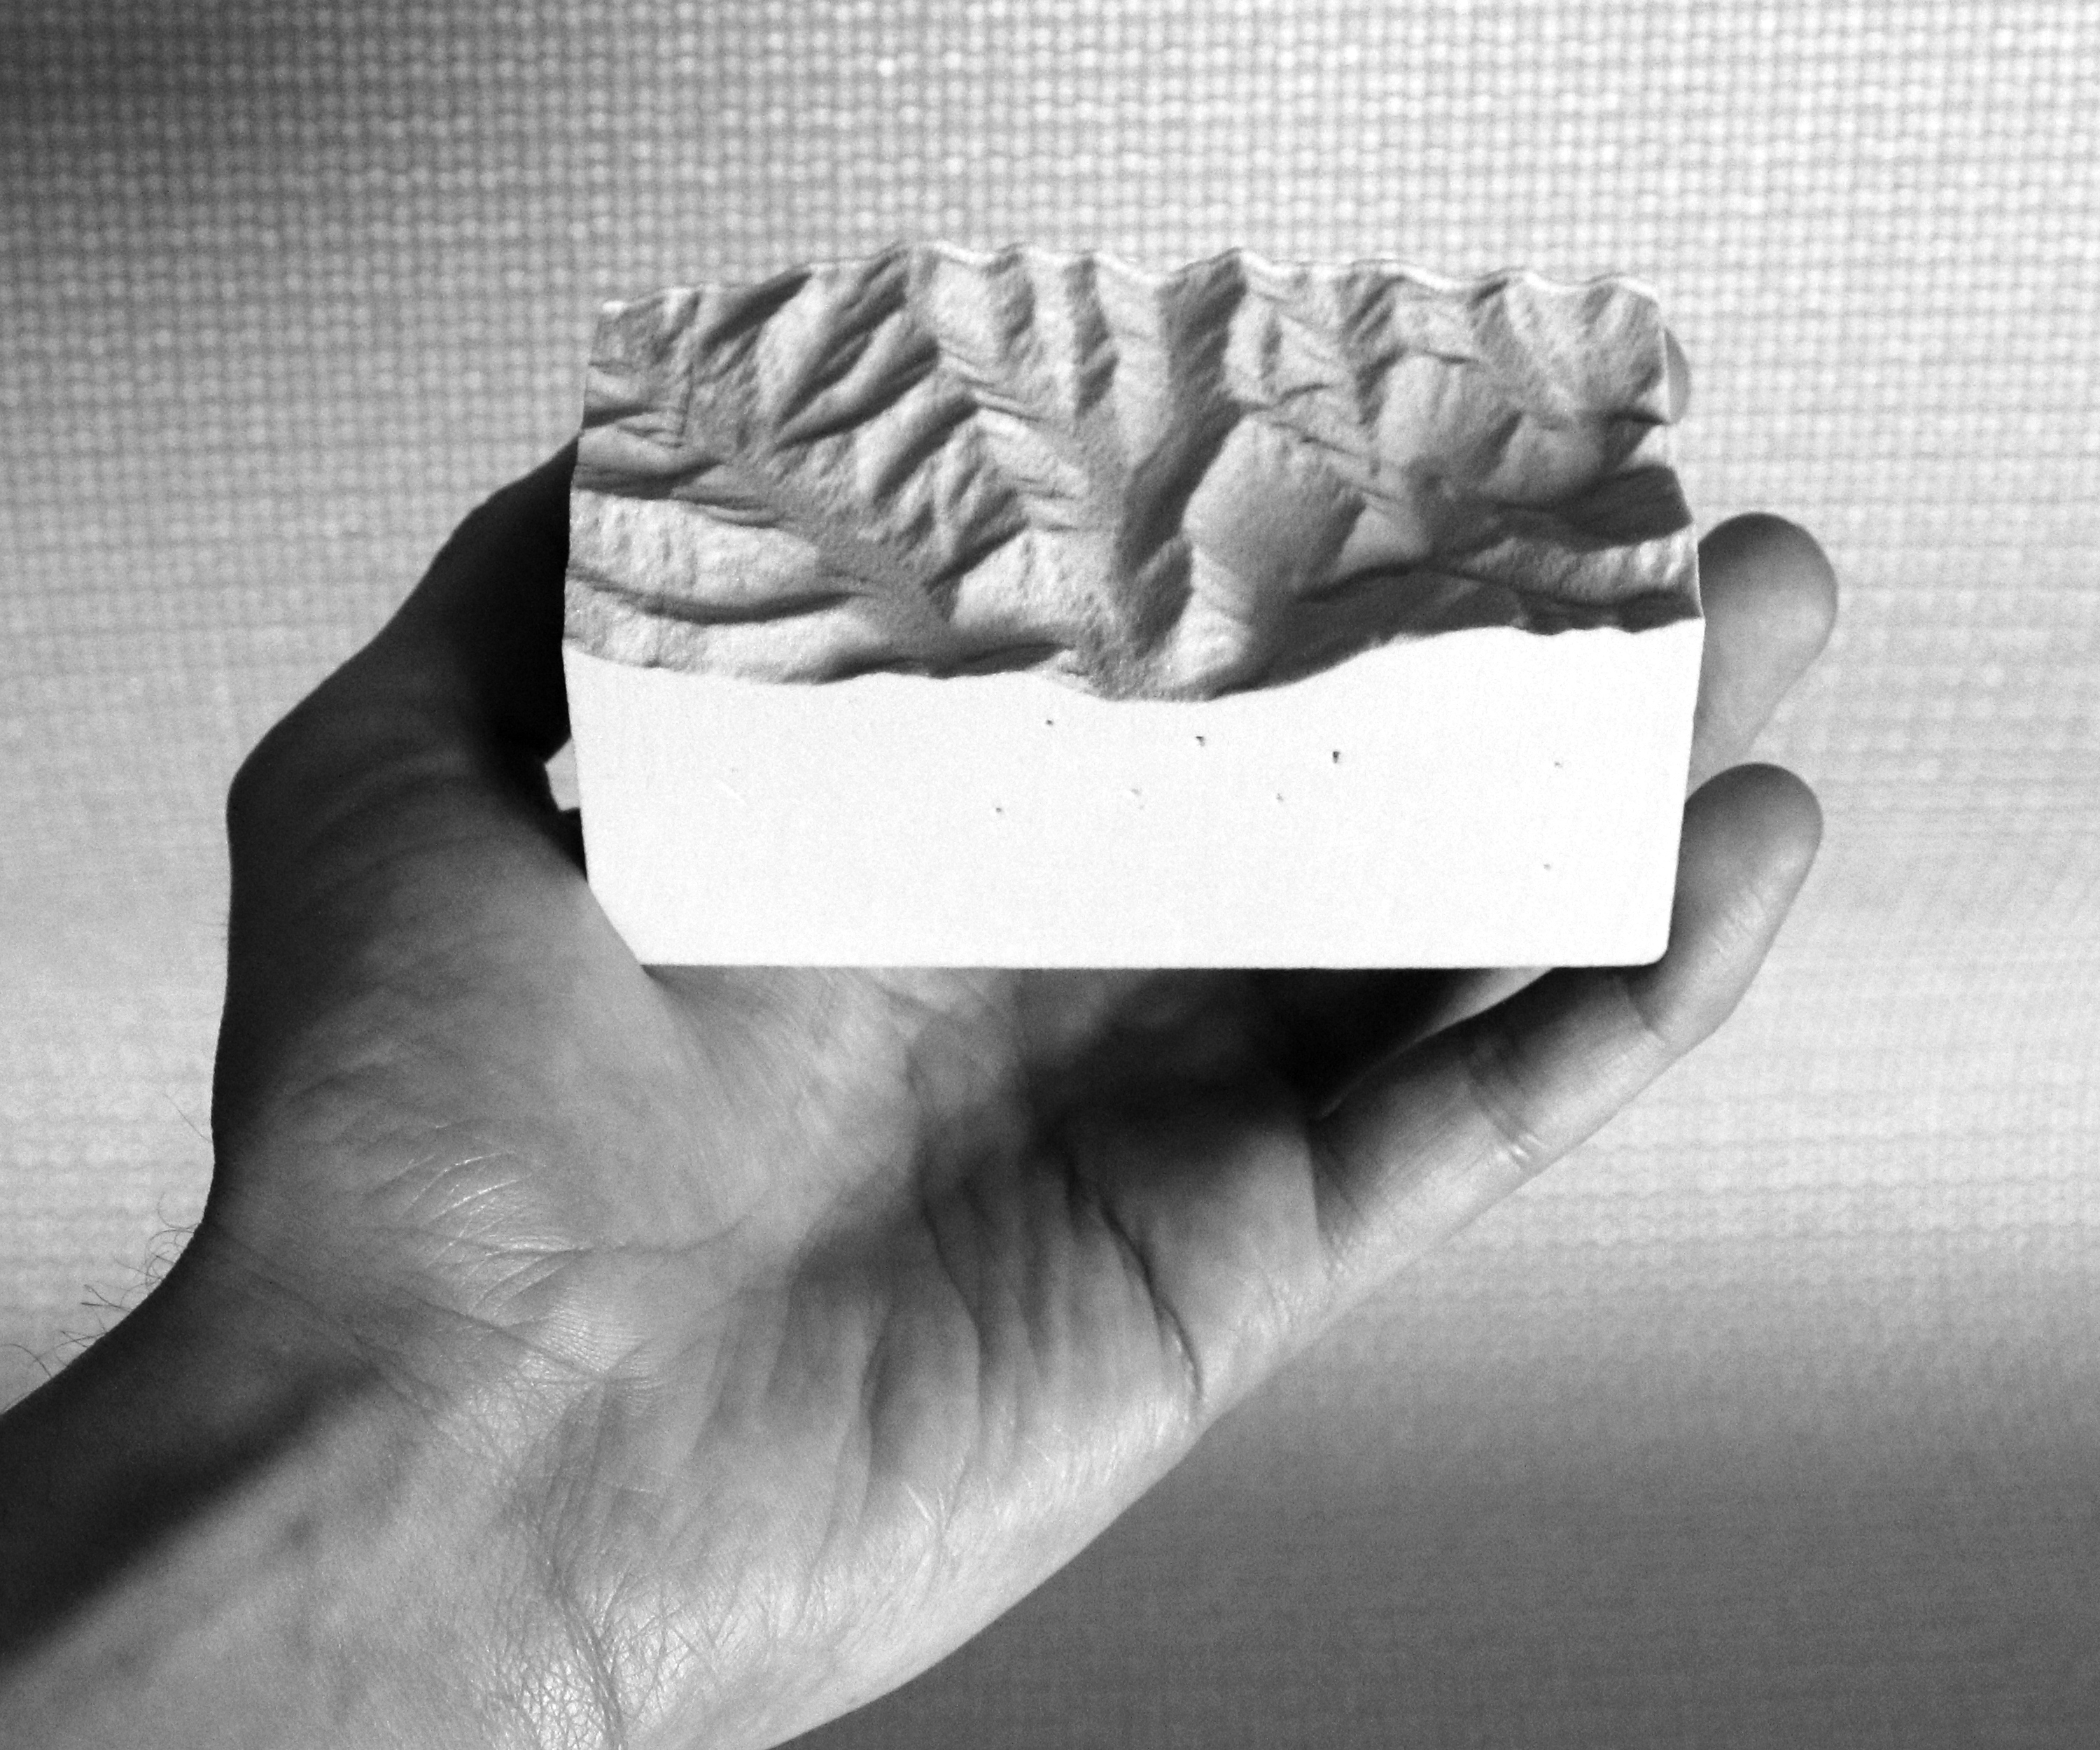
\includegraphics[width=0.49\textwidth]{images/physical_rotation_1.jpg}
%		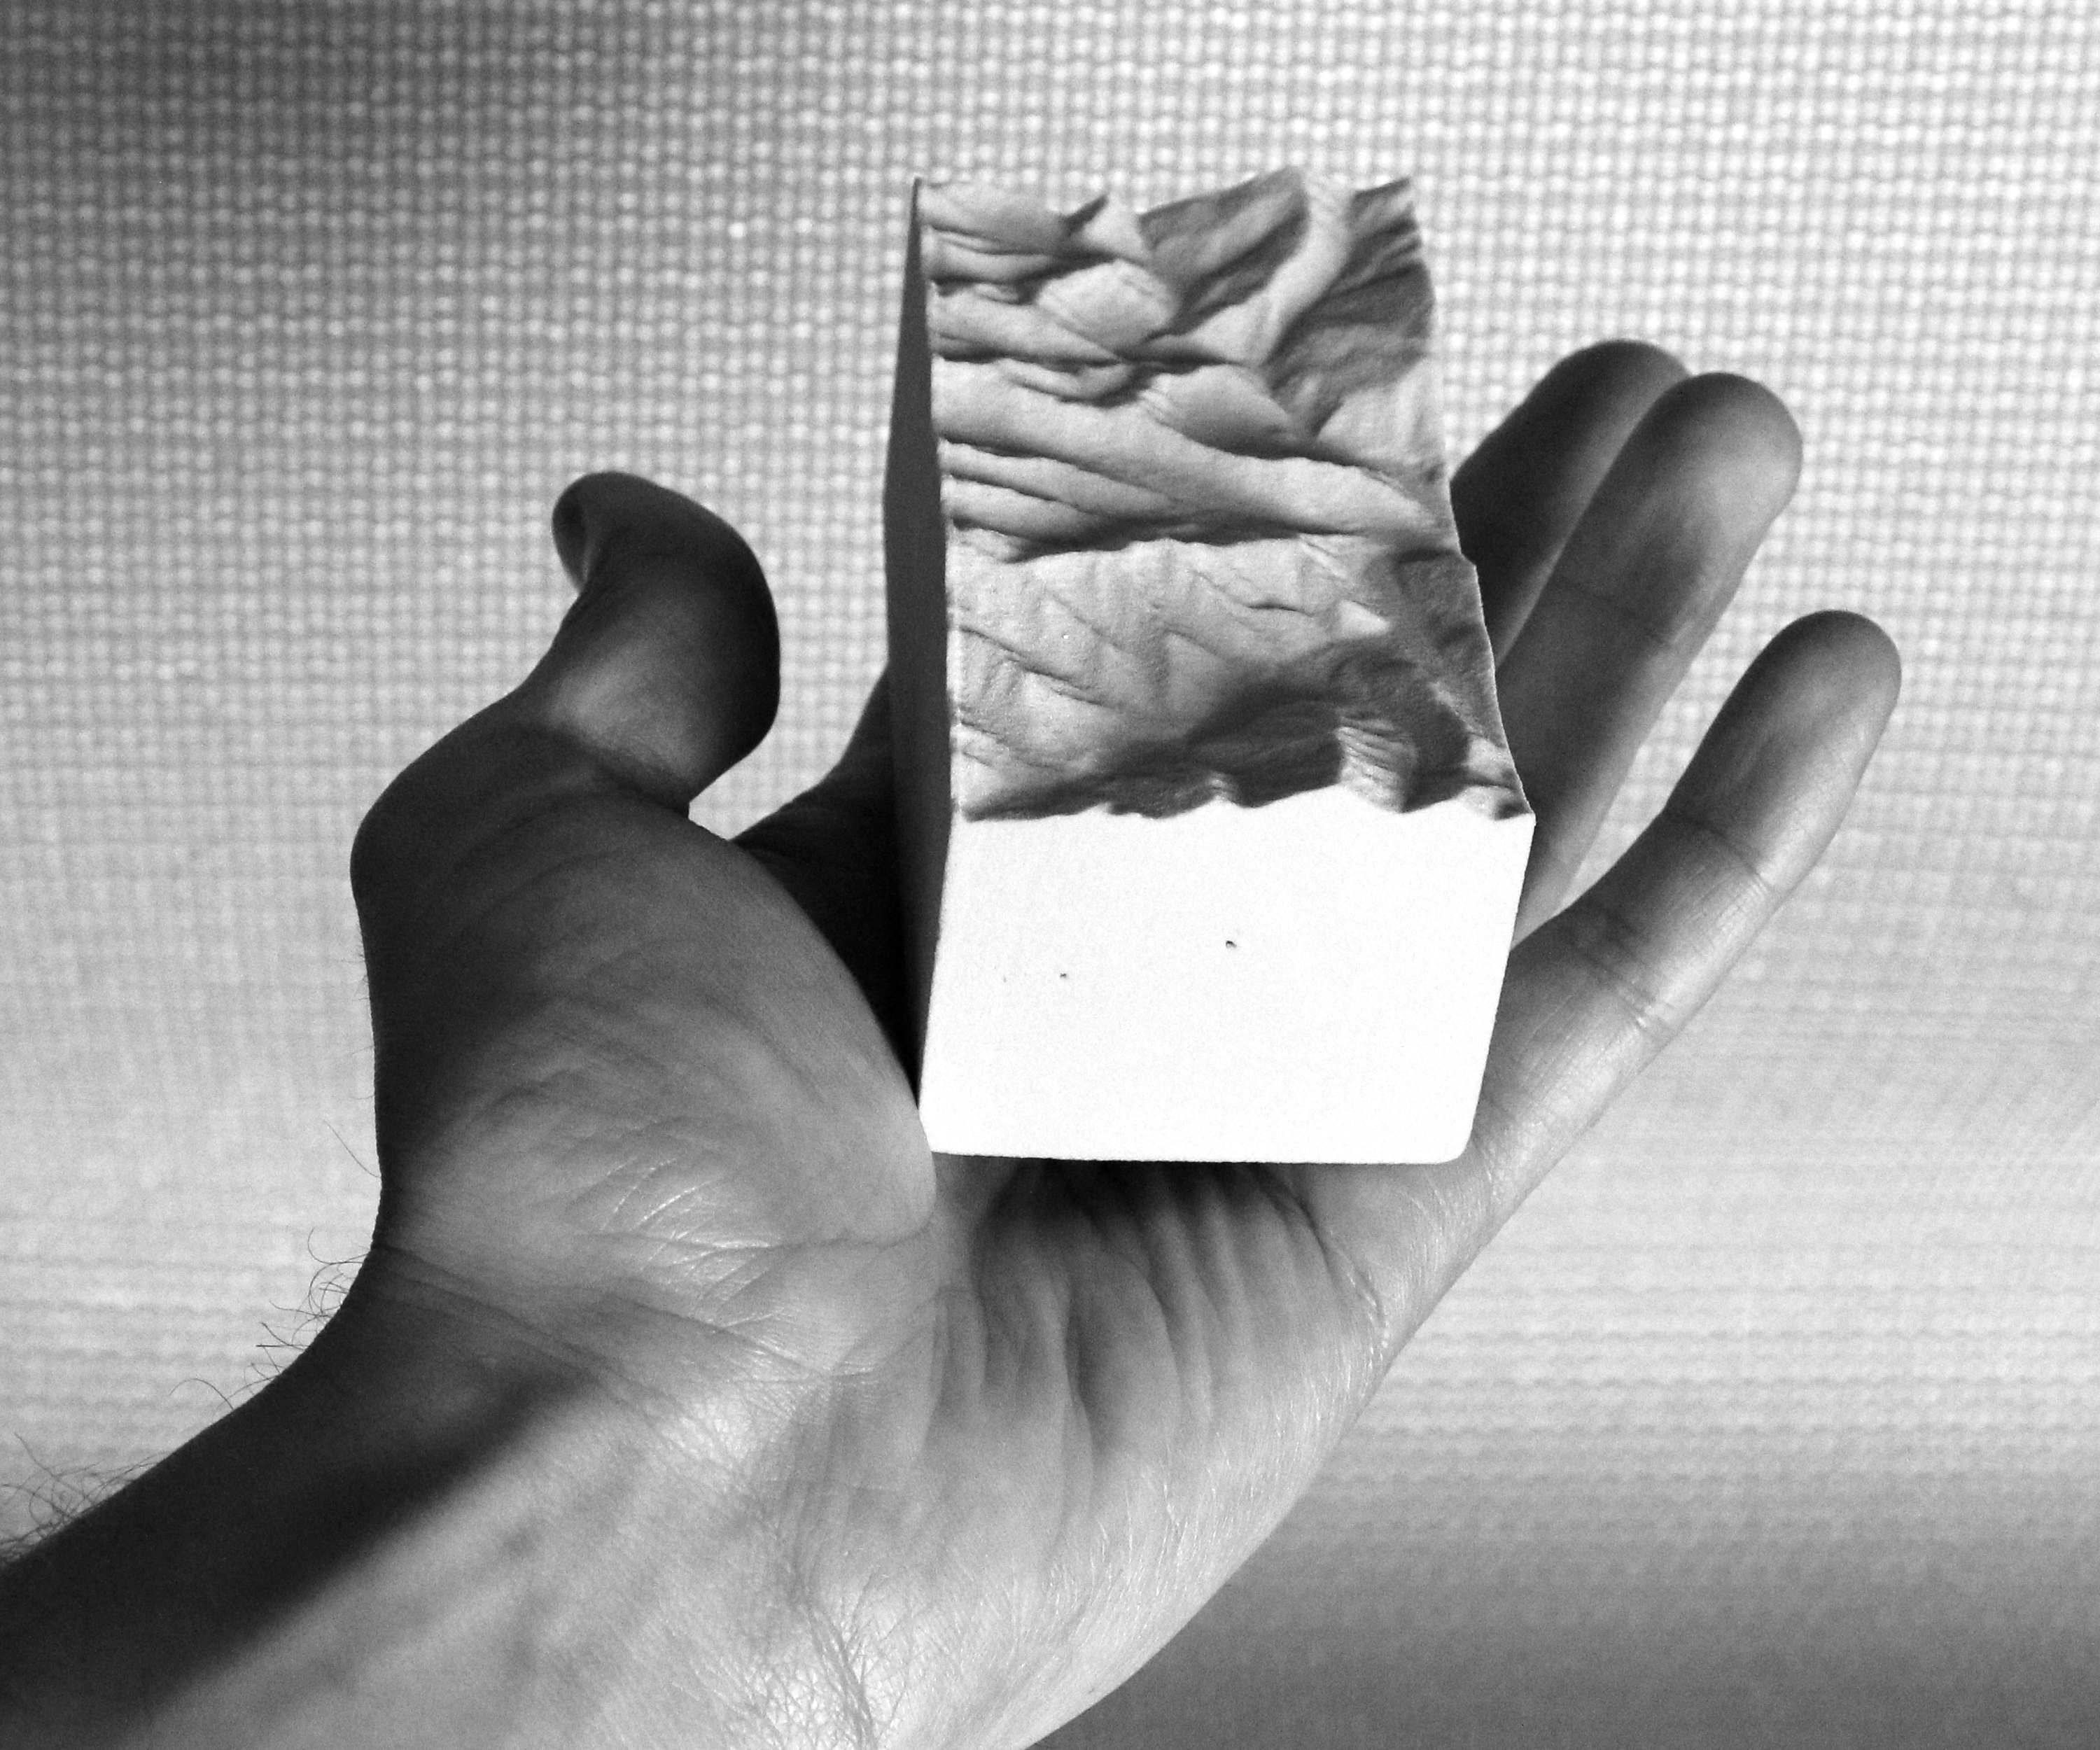
\includegraphics[width=0.49\textwidth]{images/physical_rotation_2.jpg}
%	\caption{Physically rotating a topographic model.}
%	\label{fig:physical_rotation}
%\end{center}
%\end{figure}
%
%% Physical simulation
%Furthermore, some cognitive processes can be physically simulated, offloading cognitive work onto the body \cite{Kirsh2013}. 
%%
%Mental models can be abstracted and physically simulated 
%through acting, 
%sketching, 
%or experimental adaptation or transformation. 
%%
%Kirsh cites dancers use of marking 
%-- a simplified, abstraction of a dance phrase -- 
%to learn and practice elements or aspects of the phrase \cite{Kirsh2013}. 
%%


%% Form finding
%Metacognition -- thinking about thinking -- 
%can play an important role in embodied spatial performance.
%%
%Physical simulation guided by metacognitive reflection 
%is used in generative, creative processes 
%such as sculptural form-finding or gestural sketching. 
%%
%Professionals like designers develop creative ideas through `reflection-in-action,' 
%an iterative, exploratory, metacognitive process 
%of framing a problem, ideation or making, and critical reflection \cite{Schon1983}.
%This exploratory process may unfold in an instant, 
%repeated continually throughout acts such as drawing, sculpting, and modeling. 
%%
%The architect Frank Gehry for example develops his designs through exploratory form finding with massing models
%and by thinking through the movement of gestural drawing
%\cite{Gehry2004,Pollack2006}.
%%
%An ethnography of the Office of Metropolitan Architecture
%showed that architects in the firm used exploratory modeling
%to develop designs through iterative processes
%-- exploring form by carving foam massing models with hot-wire cutters, reflecting on each model as they carved, while building up a library of forms \cite{Yaneva2009}.

%% Metacognition in tangible interaction
%Tangible interfaces enable embodied interaction
%-- the kinaesthetic exploration and physical transformation of digital data.
%%
%By embodying interaction
%users should be able to offload 
%challenging cognitive tasks 
%like sensing form, manipulating form, and imagining new forms 
%onto the body
%-- freeing up more cognitive resources for  
%metacognition. 
%%
%With more resources for metacognition
%users should be better able to parse and learn from computations.